\section{Introduction}

The intimate relationship between the environment and cellular growth rate
has remained a major topic of inquiry in bacterial physiology for over a
century. 

\begin{figure}
    \centering{
    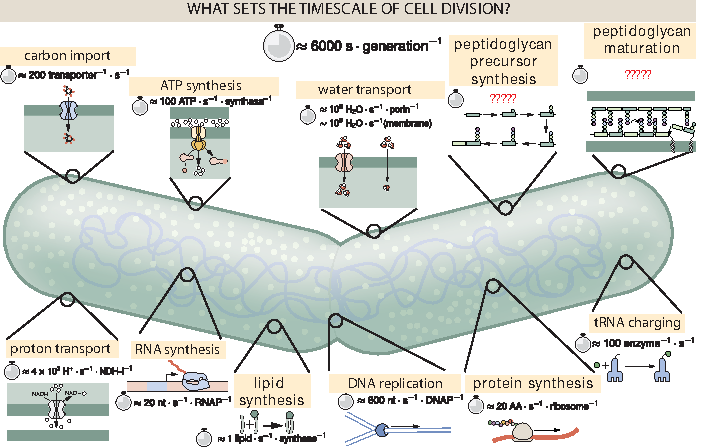
\includegraphics{../../figures/categories.pdf}
    \caption{\textbf{Transport and synthesis processes necessary for cell division.}}
    \label{fig:categories}
    }
\end{figure}



Points to emphasize
\begin{itemize}
\item The past decade of work in proteomics has made high-througput absolute
measurement of protein abundance a reality. Recent groups have used mass
spectrometry and ribosomal profiling to quantify growth-dependent effects on
protein copy numbers across growth conditions. In this work, we assemble four
recent datasets that examine how cellular proteome is influenced by the total
growth rate. 
\end{itemize}